% Options for packages loaded elsewhere
% Options for packages loaded elsewhere
\PassOptionsToPackage{unicode}{hyperref}
\PassOptionsToPackage{hyphens}{url}
\PassOptionsToPackage{dvipsnames,svgnames,x11names}{xcolor}
%
\documentclass[
  letterpaper,
  DIV=11,
  numbers=noendperiod]{scrartcl}
\usepackage{xcolor}
\usepackage{amsmath,amssymb}
\setcounter{secnumdepth}{-\maxdimen} % remove section numbering
\usepackage{iftex}
\ifPDFTeX
  \usepackage[T1]{fontenc}
  \usepackage[utf8]{inputenc}
  \usepackage{textcomp} % provide euro and other symbols
\else % if luatex or xetex
  \usepackage{unicode-math} % this also loads fontspec
  \defaultfontfeatures{Scale=MatchLowercase}
  \defaultfontfeatures[\rmfamily]{Ligatures=TeX,Scale=1}
\fi
\usepackage{lmodern}
\ifPDFTeX\else
  % xetex/luatex font selection
\fi
% Use upquote if available, for straight quotes in verbatim environments
\IfFileExists{upquote.sty}{\usepackage{upquote}}{}
\IfFileExists{microtype.sty}{% use microtype if available
  \usepackage[]{microtype}
  \UseMicrotypeSet[protrusion]{basicmath} % disable protrusion for tt fonts
}{}
\makeatletter
\@ifundefined{KOMAClassName}{% if non-KOMA class
  \IfFileExists{parskip.sty}{%
    \usepackage{parskip}
  }{% else
    \setlength{\parindent}{0pt}
    \setlength{\parskip}{6pt plus 2pt minus 1pt}}
}{% if KOMA class
  \KOMAoptions{parskip=half}}
\makeatother
% Make \paragraph and \subparagraph free-standing
\makeatletter
\ifx\paragraph\undefined\else
  \let\oldparagraph\paragraph
  \renewcommand{\paragraph}{
    \@ifstar
      \xxxParagraphStar
      \xxxParagraphNoStar
  }
  \newcommand{\xxxParagraphStar}[1]{\oldparagraph*{#1}\mbox{}}
  \newcommand{\xxxParagraphNoStar}[1]{\oldparagraph{#1}\mbox{}}
\fi
\ifx\subparagraph\undefined\else
  \let\oldsubparagraph\subparagraph
  \renewcommand{\subparagraph}{
    \@ifstar
      \xxxSubParagraphStar
      \xxxSubParagraphNoStar
  }
  \newcommand{\xxxSubParagraphStar}[1]{\oldsubparagraph*{#1}\mbox{}}
  \newcommand{\xxxSubParagraphNoStar}[1]{\oldsubparagraph{#1}\mbox{}}
\fi
\makeatother

\usepackage{color}
\usepackage{fancyvrb}
\newcommand{\VerbBar}{|}
\newcommand{\VERB}{\Verb[commandchars=\\\{\}]}
\DefineVerbatimEnvironment{Highlighting}{Verbatim}{commandchars=\\\{\}}
% Add ',fontsize=\small' for more characters per line
\usepackage{framed}
\definecolor{shadecolor}{RGB}{241,243,245}
\newenvironment{Shaded}{\begin{snugshade}}{\end{snugshade}}
\newcommand{\AlertTok}[1]{\textcolor[rgb]{0.68,0.00,0.00}{#1}}
\newcommand{\AnnotationTok}[1]{\textcolor[rgb]{0.37,0.37,0.37}{#1}}
\newcommand{\AttributeTok}[1]{\textcolor[rgb]{0.40,0.45,0.13}{#1}}
\newcommand{\BaseNTok}[1]{\textcolor[rgb]{0.68,0.00,0.00}{#1}}
\newcommand{\BuiltInTok}[1]{\textcolor[rgb]{0.00,0.23,0.31}{#1}}
\newcommand{\CharTok}[1]{\textcolor[rgb]{0.13,0.47,0.30}{#1}}
\newcommand{\CommentTok}[1]{\textcolor[rgb]{0.37,0.37,0.37}{#1}}
\newcommand{\CommentVarTok}[1]{\textcolor[rgb]{0.37,0.37,0.37}{\textit{#1}}}
\newcommand{\ConstantTok}[1]{\textcolor[rgb]{0.56,0.35,0.01}{#1}}
\newcommand{\ControlFlowTok}[1]{\textcolor[rgb]{0.00,0.23,0.31}{\textbf{#1}}}
\newcommand{\DataTypeTok}[1]{\textcolor[rgb]{0.68,0.00,0.00}{#1}}
\newcommand{\DecValTok}[1]{\textcolor[rgb]{0.68,0.00,0.00}{#1}}
\newcommand{\DocumentationTok}[1]{\textcolor[rgb]{0.37,0.37,0.37}{\textit{#1}}}
\newcommand{\ErrorTok}[1]{\textcolor[rgb]{0.68,0.00,0.00}{#1}}
\newcommand{\ExtensionTok}[1]{\textcolor[rgb]{0.00,0.23,0.31}{#1}}
\newcommand{\FloatTok}[1]{\textcolor[rgb]{0.68,0.00,0.00}{#1}}
\newcommand{\FunctionTok}[1]{\textcolor[rgb]{0.28,0.35,0.67}{#1}}
\newcommand{\ImportTok}[1]{\textcolor[rgb]{0.00,0.46,0.62}{#1}}
\newcommand{\InformationTok}[1]{\textcolor[rgb]{0.37,0.37,0.37}{#1}}
\newcommand{\KeywordTok}[1]{\textcolor[rgb]{0.00,0.23,0.31}{\textbf{#1}}}
\newcommand{\NormalTok}[1]{\textcolor[rgb]{0.00,0.23,0.31}{#1}}
\newcommand{\OperatorTok}[1]{\textcolor[rgb]{0.37,0.37,0.37}{#1}}
\newcommand{\OtherTok}[1]{\textcolor[rgb]{0.00,0.23,0.31}{#1}}
\newcommand{\PreprocessorTok}[1]{\textcolor[rgb]{0.68,0.00,0.00}{#1}}
\newcommand{\RegionMarkerTok}[1]{\textcolor[rgb]{0.00,0.23,0.31}{#1}}
\newcommand{\SpecialCharTok}[1]{\textcolor[rgb]{0.37,0.37,0.37}{#1}}
\newcommand{\SpecialStringTok}[1]{\textcolor[rgb]{0.13,0.47,0.30}{#1}}
\newcommand{\StringTok}[1]{\textcolor[rgb]{0.13,0.47,0.30}{#1}}
\newcommand{\VariableTok}[1]{\textcolor[rgb]{0.07,0.07,0.07}{#1}}
\newcommand{\VerbatimStringTok}[1]{\textcolor[rgb]{0.13,0.47,0.30}{#1}}
\newcommand{\WarningTok}[1]{\textcolor[rgb]{0.37,0.37,0.37}{\textit{#1}}}

\usepackage{longtable,booktabs,array}
\usepackage{calc} % for calculating minipage widths
% Correct order of tables after \paragraph or \subparagraph
\usepackage{etoolbox}
\makeatletter
\patchcmd\longtable{\par}{\if@noskipsec\mbox{}\fi\par}{}{}
\makeatother
% Allow footnotes in longtable head/foot
\IfFileExists{footnotehyper.sty}{\usepackage{footnotehyper}}{\usepackage{footnote}}
\makesavenoteenv{longtable}
\usepackage{graphicx}
\makeatletter
\newsavebox\pandoc@box
\newcommand*\pandocbounded[1]{% scales image to fit in text height/width
  \sbox\pandoc@box{#1}%
  \Gscale@div\@tempa{\textheight}{\dimexpr\ht\pandoc@box+\dp\pandoc@box\relax}%
  \Gscale@div\@tempb{\linewidth}{\wd\pandoc@box}%
  \ifdim\@tempb\p@<\@tempa\p@\let\@tempa\@tempb\fi% select the smaller of both
  \ifdim\@tempa\p@<\p@\scalebox{\@tempa}{\usebox\pandoc@box}%
  \else\usebox{\pandoc@box}%
  \fi%
}
% Set default figure placement to htbp
\def\fps@figure{htbp}
\makeatother


% definitions for citeproc citations
\NewDocumentCommand\citeproctext{}{}
\NewDocumentCommand\citeproc{mm}{%
  \begingroup\def\citeproctext{#2}\cite{#1}\endgroup}
\makeatletter
 % allow citations to break across lines
 \let\@cite@ofmt\@firstofone
 % avoid brackets around text for \cite:
 \def\@biblabel#1{}
 \def\@cite#1#2{{#1\if@tempswa , #2\fi}}
\makeatother
\newlength{\cslhangindent}
\setlength{\cslhangindent}{1.5em}
\newlength{\csllabelwidth}
\setlength{\csllabelwidth}{3em}
\newenvironment{CSLReferences}[2] % #1 hanging-indent, #2 entry-spacing
 {\begin{list}{}{%
  \setlength{\itemindent}{0pt}
  \setlength{\leftmargin}{0pt}
  \setlength{\parsep}{0pt}
  % turn on hanging indent if param 1 is 1
  \ifodd #1
   \setlength{\leftmargin}{\cslhangindent}
   \setlength{\itemindent}{-1\cslhangindent}
  \fi
  % set entry spacing
  \setlength{\itemsep}{#2\baselineskip}}}
 {\end{list}}
\usepackage{calc}
\newcommand{\CSLBlock}[1]{\hfill\break\parbox[t]{\linewidth}{\strut\ignorespaces#1\strut}}
\newcommand{\CSLLeftMargin}[1]{\parbox[t]{\csllabelwidth}{\strut#1\strut}}
\newcommand{\CSLRightInline}[1]{\parbox[t]{\linewidth - \csllabelwidth}{\strut#1\strut}}
\newcommand{\CSLIndent}[1]{\hspace{\cslhangindent}#1}



\setlength{\emergencystretch}{3em} % prevent overfull lines

\providecommand{\tightlist}{%
  \setlength{\itemsep}{0pt}\setlength{\parskip}{0pt}}



 


\usepackage{booktabs}
\usepackage{longtable}
\usepackage{array}
\usepackage{multirow}
\usepackage{wrapfig}
\usepackage{float}
\usepackage{colortbl}
\usepackage{pdflscape}
\usepackage{tabu}
\usepackage{threeparttable}
\usepackage{threeparttablex}
\usepackage[normalem]{ulem}
\usepackage{makecell}
\usepackage{xcolor}
\usepackage{colortbl}
\usepackage{xcolor}
\KOMAoption{captions}{tableheading}
\makeatletter
\@ifpackageloaded{caption}{}{\usepackage{caption}}
\AtBeginDocument{%
\ifdefined\contentsname
  \renewcommand*\contentsname{Table of contents}
\else
  \newcommand\contentsname{Table of contents}
\fi
\ifdefined\listfigurename
  \renewcommand*\listfigurename{List of Figures}
\else
  \newcommand\listfigurename{List of Figures}
\fi
\ifdefined\listtablename
  \renewcommand*\listtablename{List of Tables}
\else
  \newcommand\listtablename{List of Tables}
\fi
\ifdefined\figurename
  \renewcommand*\figurename{Figure}
\else
  \newcommand\figurename{Figure}
\fi
\ifdefined\tablename
  \renewcommand*\tablename{Table}
\else
  \newcommand\tablename{Table}
\fi
}
\@ifpackageloaded{float}{}{\usepackage{float}}
\floatstyle{ruled}
\@ifundefined{c@chapter}{\newfloat{codelisting}{h}{lop}}{\newfloat{codelisting}{h}{lop}[chapter]}
\floatname{codelisting}{Listing}
\newcommand*\listoflistings{\listof{codelisting}{List of Listings}}
\makeatother
\makeatletter
\makeatother
\makeatletter
\@ifpackageloaded{caption}{}{\usepackage{caption}}
\@ifpackageloaded{subcaption}{}{\usepackage{subcaption}}
\makeatother
\usepackage{bookmark}
\IfFileExists{xurl.sty}{\usepackage{xurl}}{} % add URL line breaks if available
\urlstyle{same}
\hypersetup{
  pdftitle={ECON-S307 Séminaire d'économie appliquée - Prix},
  pdfauthor={Owen Brown},
  colorlinks=true,
  linkcolor={blue},
  filecolor={Maroon},
  citecolor={Blue},
  urlcolor={Blue},
  pdfcreator={LaTeX via pandoc}}


\title{ECON-S307 Séminaire d'économie appliquée - Prix}
\usepackage{etoolbox}
\makeatletter
\providecommand{\subtitle}[1]{% add subtitle to \maketitle
  \apptocmd{\@title}{\par {\large #1 \par}}{}{}
}
\makeatother
\subtitle{Séance d'introduction}
\author{Owen Brown}
\date{February 6, 2026}
\begin{document}
\maketitle


\begin{Shaded}
\begin{Highlighting}[]
\FunctionTok{source}\NormalTok{(}\StringTok{"lib.R"}\NormalTok{)}
\FunctionTok{source}\NormalTok{(}\StringTok{"data\_forProj.R"}\NormalTok{)}
\FunctionTok{set.seed}\NormalTok{(}\DecValTok{1234}\NormalTok{)}
\NormalTok{puissance }\OtherTok{\textless{}{-}} \FunctionTok{rnorm}\NormalTok{(}\DecValTok{5000}\NormalTok{,}\DecValTok{200}\NormalTok{,}\DecValTok{75}\NormalTok{)}
\NormalTok{poids }\OtherTok{\textless{}{-}} \FunctionTok{rnorm}\NormalTok{(}\DecValTok{5000}\NormalTok{,}\DecValTok{500}\NormalTok{,}\DecValTok{250}\NormalTok{)}\SpecialCharTok{+}\FloatTok{0.2}\SpecialCharTok{*}\NormalTok{puissance}

\NormalTok{prix }\OtherTok{\textless{}{-}} \DecValTok{3500}\FloatTok{+0.5}\SpecialCharTok{*}\NormalTok{puissance}\DecValTok{{-}1}\SpecialCharTok{*}\NormalTok{poids}\SpecialCharTok{+}\FunctionTok{rnorm}\NormalTok{(}\DecValTok{5000}\NormalTok{,}\DecValTok{150}\NormalTok{,}\DecValTok{100}\NormalTok{)}

\NormalTok{dta }\OtherTok{\textless{}{-}} \FunctionTok{tibble}\NormalTok{(prix,puissance,poids)}

\NormalTok{fmla }\OtherTok{\textless{}{-}}\NormalTok{ prix}\SpecialCharTok{\textasciitilde{}} \DecValTok{1000}\FloatTok{+0.5}\SpecialCharTok{*}\NormalTok{puissance}\FloatTok{{-}0.10}\SpecialCharTok{*}\NormalTok{poids}

\CommentTok{\#| include: false}
\NormalTok{knitr}\SpecialCharTok{::}\NormalTok{opts\_chunk}\SpecialCharTok{$}\FunctionTok{set}\NormalTok{(}\AttributeTok{warning =} \ConstantTok{FALSE}\NormalTok{,}
  \AttributeTok{error   =} \ConstantTok{FALSE}
\NormalTok{)}
\end{Highlighting}
\end{Shaded}

\subsection{Objectif de la séance}\label{objectif-de-la-suxe9ance}

L'objectif de cette séance sera de revenir sur l'organisation du cours
et du matériel que nous emploierons. Nous discuterons:

\begin{itemize}
\tightlist
\item
  de l'objectif général du projet
\item
  des outils mobilisables pour ce projet
\item
  du travail final à rendre
\end{itemize}

\subsection{Structure du projet}\label{structure-du-projet}

Chaque groupe doit rédiger un projet de 4 pages / membre (page de garde,
appendix et références exclues - taille de police 12). Le projet doit
prendre la forme suivante :

\begin{enumerate}
\def\labelenumi{\arabic{enumi}.}
\setcounter{enumi}{-1}
\tightlist
\item
  \textbf{Page de garde} - titre, noms, matricules
\item
  \textbf{Revue de littérature} - synthèse de la recherche relative à
  votre bien
\item
  \textbf{Discussion de la source de données} - justification,
  fiabilité,méthode de récolte
\item
  \textbf{Analyse descriptive des données} - sommaire des variables,
  graphiques, tables
\item
  \textbf{Méthode, résultats, discussion} - spécification de la
  régression hédonique, estimation de modèle, discussion des résultats,
  liens contextuels
\item
  \textbf{Références \& Appendix}
\end{enumerate}

. . .

Le travail comprendra en préambule une table de matières ainsi qu'une
table de graphiques.

\subsection{Remise \& défense de
projet}\label{remise-duxe9fense-de-projet}

\begin{itemize}
\tightlist
\item
  Votre fichier devra être remis \textbf{sur l'UV sous format PDF}.
\item
  En indiquant votre numéro de groupe et vos noms (de famille) par ordre
  alphabétique, vous nommerez votre le fichier de votre travail :
\end{itemize}

``{[}GRP\_{]} - Séminaire d'économie appliquée
(Prix)\_NOM\_1-NOM\_2-NOM\_3.pdf''.

. . .

\begin{itemize}
\tightlist
\item
  Vous devrez également soumettre votre jeu de données ainsi que votre
  code. \textbf{Il est impératif que le code que vous communiquez
  produise exactement les mêmes résultats que votre travail.}
\item
  Votre code devra être commenté. Chaque étape clé devra être clairement
  indiquée et brièvement décrite.
\end{itemize}

``{[}GRP\_{]} - Code\_NOM\_1-NOM\_2-NOM\_3.R'' ``{[}GRP\_{]} -
Dataset\_NOM\_1-NOM\_2-NOM\_3.csv''

\subsection{Dates du projet}\label{dates-du-projet}

\begin{itemize}
\tightlist
\item
  \textbf{1er mars - 23h59} : Remettre une note dans laquelle vous
  expliquez quel bien vous souhaitez analyser et expliquez comment vous
  construirez un jeu de données (1 page max).

  \emph{{[}GRP\_{]} - Note 1 (Prix)\_NOM\_1-NOM\_2-NOM\_3.pdf}
\item
  \textbf{15 mars - 23h59} : Remettre une note dans laquelle vous
  expliquez votre avancée de récolte de données - Méthode employée,
  source, quantité de données, objectifs (2 pages max).

  \emph{{[}GRP\_{]} - Note 2 (Prix)\_NOM\_1-NOM\_2-NOM\_3.pdf}
\item
  \textbf{30 avril - 23h59} : Remettre votre travail sur l'UV

  \begin{itemize}
  \tightlist
  \item
    Votre rapport final - \textbf{format PDF}
  \item
    Vos documents annexes - Jeu de données, codes
  \end{itemize}
\end{itemize}

\section{Des questions ?}\label{des-questions}

\subsection{Du projet}\label{du-projet}

\begin{enumerate}
\def\labelenumi{\arabic{enumi}.}
\tightlist
\item
  L'objectif de ce projet est de vous faire mesurer. Mesurer, c'est
  central en économie appliquée.
\item
  Votre objet d'étude sera un bien.
\item
  Vous devrez mesurer la contribution des caractéristiques d'un bien au
  prix de ce bien.
\end{enumerate}

. . .

→ Ceci peut être réalisé avec des outils économétriques : les
régressions hédoniques.

. . .

Une régression hédonique décompose le prix en ses constituants
caractéristiques, et fournit une estimation de la valeur contributaire
de chaque caractéristique.

\subsection{\texorpdfstring{Rappel - L'économétrie {Wooldridge
(2015)}}{Rappel - L'économétrie Wooldridge (2015)}}\label{rappel---luxe9conomuxe9trie-woolridge}

L'économétrie est un outil fondé sur des méthodes statistiques ayant
pour but :

\begin{itemize}
\tightlist
\item
  d'estimer des relations économiques
\item
  de tester des théories
\item
  de mesurer des effets
\end{itemize}

. . .

Cet outil nous permet de mesurer la contribution d'une caractéristique
au prix d'un bien.

\subsection{Exemple}\label{exemple}

Imaginons que nous voulions estimer le prix d'une voiture selon ses
caractéristiques.

. . .

D'intuition, nous dirions que le prix de la voiture dépend de plusieurs
facteurs, notamment :

\begin{enumerate}
\def\labelenumi{\arabic{enumi}.}
\tightlist
\item
  Sa puissance (+)
\item
  Son poids (-)
\end{enumerate}

\subsection{Exemple}\label{exemple-1}

Faisant l'hypothèse que la relation entre le prix et les
caractéristiques prend une forme fonctionelle suivante:

\begin{equation}
Prix_i =  \beta_1 \cdot Puissance_i  + \beta_2 \cdot Poids_i
\end{equation}

. . .

L'économétrie nous permet d'estimer les coefficients \(\beta\).

. . .

Si notre intuition s'avère correcte, une OLS délivrerait des estimations
telles que :

\begin{itemize}
\tightlist
\item
  \(\hat{\beta_1}>0\)
\item
  \(\hat{\beta_2}<0\)
\end{itemize}

\subsection{Données}\label{donnuxe9es}

Soit un jeu de données à notre disposition:

\begin{Shaded}
\begin{Highlighting}[]
\NormalTok{dta }\SpecialCharTok{\%\textgreater{}\%} \FunctionTok{select}\NormalTok{(}\FunctionTok{c}\NormalTok{(}\StringTok{"prix"}\NormalTok{,}\StringTok{"puissance"}\NormalTok{,}\StringTok{"poids"}\NormalTok{)) }\SpecialCharTok{\%\textgreater{}\%}\NormalTok{ summary}
\end{Highlighting}
\end{Shaded}

\begin{verbatim}
      prix        puissance         poids       
 Min.   :2172   Min.   :-54.7   Min.   :-308.1  
 1st Qu.:3030   1st Qu.:149.3   1st Qu.: 380.8  
 Median :3200   Median :199.6   Median : 542.5  
 Mean   :3206   Mean   :199.5   Mean   : 544.6  
 3rd Qu.:3381   3rd Qu.:249.9   3rd Qu.: 710.6  
 Max.   :4211   Max.   :439.7   Max.   :1446.7  
\end{verbatim}

\begin{Shaded}
\begin{Highlighting}[]
\NormalTok{dta }\SpecialCharTok{\%\textgreater{}\%} \FunctionTok{select}\NormalTok{(}\FunctionTok{c}\NormalTok{(}\StringTok{"prix"}\NormalTok{,}\StringTok{"puissance"}\NormalTok{,}\StringTok{"poids"}\NormalTok{)) }\SpecialCharTok{\%\textgreater{}\%}\NormalTok{ dim}
\end{Highlighting}
\end{Shaded}

\begin{verbatim}
[1] 5000    3
\end{verbatim}

\subsection{Testons notre modèle}\label{testons-notre-moduxe8le}

Une estimation par la méthode des moindres carrés (OLS) nous donne:

\begin{Shaded}
\begin{Highlighting}[]
\NormalTok{reg }\OtherTok{\textless{}{-}}\NormalTok{ dta }\SpecialCharTok{\%\textgreater{}\%} \FunctionTok{lm}\NormalTok{(}\AttributeTok{formula=}\NormalTok{ prix }\SpecialCharTok{\textasciitilde{}}\NormalTok{poids}\SpecialCharTok{+}\NormalTok{ puissance}\DecValTok{{-}1}\NormalTok{)  }
\NormalTok{reg }\SpecialCharTok{\%\textgreater{}\%}\NormalTok{ tidy }\SpecialCharTok{\%\textgreater{}\%} \FunctionTok{kbl}\NormalTok{() }\SpecialCharTok{\%\textgreater{}\%} \FunctionTok{kable\_styling}\NormalTok{(}\AttributeTok{font\_size =} \DecValTok{35}\NormalTok{) }
\end{Highlighting}
\end{Shaded}

\begin{verbatim}
Warning in attr(.knitEnv$meta, "knit_meta_id"): 'xfun::attr()' is deprecated.
Use 'xfun::attr2()' instead.
See help("Deprecated")
Warning in attr(.knitEnv$meta, "knit_meta_id"): 'xfun::attr()' is deprecated.
Use 'xfun::attr2()' instead.
See help("Deprecated")
Warning in attr(.knitEnv$meta, "knit_meta_id"): 'xfun::attr()' is deprecated.
Use 'xfun::attr2()' instead.
See help("Deprecated")
Warning in attr(.knitEnv$meta, "knit_meta_id"): 'xfun::attr()' is deprecated.
Use 'xfun::attr2()' instead.
See help("Deprecated")
Warning in attr(.knitEnv$meta, "knit_meta_id"): 'xfun::attr()' is deprecated.
Use 'xfun::attr2()' instead.
See help("Deprecated")
Warning in attr(.knitEnv$meta, "knit_meta_id"): 'xfun::attr()' is deprecated.
Use 'xfun::attr2()' instead.
See help("Deprecated")
Warning in attr(.knitEnv$meta, "knit_meta_id"): 'xfun::attr()' is deprecated.
Use 'xfun::attr2()' instead.
See help("Deprecated")
Warning in attr(.knitEnv$meta, "knit_meta_id"): 'xfun::attr()' is deprecated.
Use 'xfun::attr2()' instead.
See help("Deprecated")
Warning in attr(.knitEnv$meta, "knit_meta_id"): 'xfun::attr()' is deprecated.
Use 'xfun::attr2()' instead.
See help("Deprecated")
Warning in attr(.knitEnv$meta, "knit_meta_id"): 'xfun::attr()' is deprecated.
Use 'xfun::attr2()' instead.
See help("Deprecated")
Warning in attr(.knitEnv$meta, "knit_meta_id"): 'xfun::attr()' is deprecated.
Use 'xfun::attr2()' instead.
See help("Deprecated")
Warning in attr(.knitEnv$meta, "knit_meta_id"): 'xfun::attr()' is deprecated.
Use 'xfun::attr2()' instead.
See help("Deprecated")
Warning in attr(.knitEnv$meta, "knit_meta_id"): 'xfun::attr()' is deprecated.
Use 'xfun::attr2()' instead.
See help("Deprecated")
Warning in attr(.knitEnv$meta, "knit_meta_id"): 'xfun::attr()' is deprecated.
Use 'xfun::attr2()' instead.
See help("Deprecated")
\end{verbatim}

\begin{verbatim}
Warning in attr(x, "align"): 'xfun::attr()' is deprecated.
Use 'xfun::attr2()' instead.
See help("Deprecated")
\end{verbatim}

\begin{verbatim}
Warning in attr(x, "format"): 'xfun::attr()' is deprecated.
Use 'xfun::attr2()' instead.
See help("Deprecated")
\end{verbatim}

\begin{table}
\centering\begingroup\fontsize{35}{37}\selectfont

\begin{tabular}[t]{l|r|r|r|r}
\hline
term & estimate & std.error & statistic & p.value\\
\hline
poids & 1.41737 & 0.0501524 & 28.26127 & 0\\
\hline
puissance & 10.68017 & 0.1408273 & 75.83878 & 0\\
\hline
\end{tabular}
\endgroup{}
\end{table}

. . .

Les deux variables ont un effet positif sur le prix. Les p-valeurs sont
significatives à plus de 99\% de confiance !

\subsection{Réfléchir à sa
modélisation}\label{ruxe9fluxe9chir-uxe0-sa-moduxe9lisation}

\begin{itemize}
\tightlist
\item
  Nos estimations contredisent notre hypothèse
  (\(\hat{\beta}_{poids}>0\)). Est-ce que nos résultats ont du sens ?
\item
  Représentons nos données
\end{itemize}

. . .

\pandocbounded{\includegraphics[keepaspectratio]{hello_files/figure-pdf/unnamed-chunk-4-1.png}}

\subsection{Revoir le modèle - I}\label{revoir-le-moduxe8le---i}

\begin{itemize}
\tightlist
\item
  Ne faudrait-il pas un intercept ? \begin{equation}
  Prix_i = \alpha_0 + \beta_1 \cdot Puissance_i  + \beta_2 \cdot Poids_i
  \end{equation}
\end{itemize}

. . .

\begin{Shaded}
\begin{Highlighting}[]
\NormalTok{reg2 }\OtherTok{\textless{}{-}}\NormalTok{ dta }\SpecialCharTok{\%\textgreater{}\%} \FunctionTok{lm}\NormalTok{(}\AttributeTok{formula=}\NormalTok{ prix }\SpecialCharTok{\textasciitilde{}}\NormalTok{poids}\SpecialCharTok{+}\NormalTok{ puissance)  }
\NormalTok{reg2 }\SpecialCharTok{\%\textgreater{}\%}\NormalTok{ tidy }\SpecialCharTok{\%\textgreater{}\%} \FunctionTok{kbl}\NormalTok{() }\SpecialCharTok{\%\textgreater{}\%} \FunctionTok{kable\_styling}\NormalTok{(}\AttributeTok{font\_size =} \DecValTok{35}\NormalTok{) }
\end{Highlighting}
\end{Shaded}

\begin{verbatim}
Warning in attr(.knitEnv$meta, "knit_meta_id"): 'xfun::attr()' is deprecated.
Use 'xfun::attr2()' instead.
See help("Deprecated")
Warning in attr(.knitEnv$meta, "knit_meta_id"): 'xfun::attr()' is deprecated.
Use 'xfun::attr2()' instead.
See help("Deprecated")
Warning in attr(.knitEnv$meta, "knit_meta_id"): 'xfun::attr()' is deprecated.
Use 'xfun::attr2()' instead.
See help("Deprecated")
Warning in attr(.knitEnv$meta, "knit_meta_id"): 'xfun::attr()' is deprecated.
Use 'xfun::attr2()' instead.
See help("Deprecated")
Warning in attr(.knitEnv$meta, "knit_meta_id"): 'xfun::attr()' is deprecated.
Use 'xfun::attr2()' instead.
See help("Deprecated")
Warning in attr(.knitEnv$meta, "knit_meta_id"): 'xfun::attr()' is deprecated.
Use 'xfun::attr2()' instead.
See help("Deprecated")
Warning in attr(.knitEnv$meta, "knit_meta_id"): 'xfun::attr()' is deprecated.
Use 'xfun::attr2()' instead.
See help("Deprecated")
Warning in attr(.knitEnv$meta, "knit_meta_id"): 'xfun::attr()' is deprecated.
Use 'xfun::attr2()' instead.
See help("Deprecated")
Warning in attr(.knitEnv$meta, "knit_meta_id"): 'xfun::attr()' is deprecated.
Use 'xfun::attr2()' instead.
See help("Deprecated")
Warning in attr(.knitEnv$meta, "knit_meta_id"): 'xfun::attr()' is deprecated.
Use 'xfun::attr2()' instead.
See help("Deprecated")
Warning in attr(.knitEnv$meta, "knit_meta_id"): 'xfun::attr()' is deprecated.
Use 'xfun::attr2()' instead.
See help("Deprecated")
Warning in attr(.knitEnv$meta, "knit_meta_id"): 'xfun::attr()' is deprecated.
Use 'xfun::attr2()' instead.
See help("Deprecated")
Warning in attr(.knitEnv$meta, "knit_meta_id"): 'xfun::attr()' is deprecated.
Use 'xfun::attr2()' instead.
See help("Deprecated")
Warning in attr(.knitEnv$meta, "knit_meta_id"): 'xfun::attr()' is deprecated.
Use 'xfun::attr2()' instead.
See help("Deprecated")
\end{verbatim}

\begin{verbatim}
Warning in attr(x, "align"): 'xfun::attr()' is deprecated.
Use 'xfun::attr2()' instead.
See help("Deprecated")
\end{verbatim}

\begin{verbatim}
Warning in attr(x, "format"): 'xfun::attr()' is deprecated.
Use 'xfun::attr2()' instead.
See help("Deprecated")
\end{verbatim}

\begin{table}
\centering\begingroup\fontsize{35}{37}\selectfont

\begin{tabular}[t]{l|r|r|r|r}
\hline
term & estimate & std.error & statistic & p.value\\
\hline
(Intercept) & 3648.7080863 & 4.8986699 & 744.83648 & 0\\
\hline
poids & -0.9992213 & 0.0057432 & -173.98399 & 0\\
\hline
puissance & 0.5064512 & 0.0190694 & 26.55832 & 0\\
\hline
\end{tabular}
\endgroup{}
\end{table}

\subsection{Revoir le modèle - II}\label{revoir-le-moduxe8le---ii}

\pandocbounded{\includegraphics[keepaspectratio]{hello_files/figure-pdf/unnamed-chunk-6-1.png}}

. . .

Beaucoup plus cohérent !

\subsection{Problème résolu ?}\label{probluxe8me-ruxe9solu}

Qu'avons nous comme outil pour évaluer s'il y a une potentielle erreur
de mesure ?

. . .

Comparons l'hétéroscédasticité (\(\sigma^2\)) des deux modèles:

\pandocbounded{\includegraphics[keepaspectratio]{hello_files/figure-pdf/unnamed-chunk-7-1.png}}

Notre second modèle semble beaucoup plus adapté.

\subsection{Remarques}\label{remarques}

\begin{itemize}
\tightlist
\item
  Une \emph{p-valeur} significative n'implique pas automatiquement que
  votre régression est correcte !
\item
  Soyez toujours critiques de votre modélisation :

  \begin{itemize}
  \tightlist
  \item
    Est-ce que mes coefficients ont du sens ?
  \item
    Ai-je à disposition un outil pour tester la véracité de mes
    résultats ?
  \end{itemize}
\item
  Codez ! Appliquer la théorie économétrique est un moyen précieux de
  rendre cette discipline plus claire.
\end{itemize}

\subsection{À vous !}\label{uxe0-vous}

\begin{itemize}
\tightlist
\item
  Pour le projet il vous sera demandé de constituer une base de données.
  Vous pouvez récolter des données où vous le désirez, \textbf{tant que
  vous obtenez un jeu de données réelles}.
\item
  Rassembler des données peut être couteux. Toutefois avec internet,vous
  avez à dispositions une masse considérable de données. Mais comment
  les réunir ?
\item
  Le webscraping !
\end{itemize}

\subsection{Le webscraping}\label{le-webscraping}

\begin{enumerate}
\def\labelenumi{\arabic{enumi}.}
\tightlist
\item
  Le \emph{webscraping} est une méthode d'extraction de données de site
  web
\item
  Cette méthode exploite la structure des pages pour récupérer
  automatiquement de l'information
\item
  Elle s'avère très efficace pour constituer rapidement un jeu important
  de données !
\item
  En revanche, parce qu'un grand nombre de données en récolté, un
  travail de nettoyage de données est souvent nécessaire
\end{enumerate}

. . .

\subsection{La structure des pages ?}\label{la-structure-des-pages}

Les sites web que nous voyons sont en réalité une interprétation de code
HTML.

\includegraphics[width=1.3\linewidth,height=\textheight,keepaspectratio]{Screen Shot 2026-02-02 at 23.42.19.png}

\includegraphics[width=0.7\linewidth,height=\textheight,keepaspectratio]{Capture d’écran 2026-02-02 234320.png}

\subsection{Scraper une page - I}\label{scraper-une-page---i}

\begin{itemize}
\tightlist
\item
  À quelques exceptions près, tous les sites web suivent un structure
  par ``balise''
\item
  Avec \texttt{R} ou \texttt{Python} et la libraire \emph{Selenium}, il
  est possible de simuler une navigation internet et d'enregister de
  l'information contenu dans un code \emph{HTML}.
\end{itemize}

\subsection{Scraper une page - II}\label{scraper-une-page---ii}

Par étape :

\begin{enumerate}
\def\labelenumi{\arabic{enumi}.}
\tightlist
\item
  Trouver une page type qui contient l'information sur le bien d'intérêt
\item
  Comprendre la structure du site
\item
  Localiser les balises d'information
\item
  Automatiser la navigation
\item
  Récolter les données et les stocker dans un fichier lisible par votre
  programme statistique
\end{enumerate}

\section{Un exemple peut-être ?}\label{un-exemple-peut-uxeatre}

\subsection{Le prix des téléphones}\label{le-prix-des-tuxe9luxe9phones}

Quels sont les éléments constitutifs des prix de téléphone ?

\begin{itemize}
\tightlist
\item
  Le stockage
\item
  La marque
\item
  L'autonomie
\item
  La performance
\end{itemize}

. . .

Créons un jeu de données !

\subsection{Jeu de donnée}\label{jeu-de-donnuxe9e}

Après la récolte automatisée ainsi que le nettoyage des données, nous
obtenons un jeu tel que suit :

\begin{Shaded}
\begin{Highlighting}[]
\NormalTok{phonesdf }\SpecialCharTok{\%\textgreater{}\%} \FunctionTok{print}\NormalTok{(}\AttributeTok{n=}\DecValTok{28}\NormalTok{)}
\end{Highlighting}
\end{Shaded}

\begin{verbatim}
# A tibble: 28 x 14
   Produit price `Qualité de la caméra` `Année d'introduction` Marque   Garantie
   <chr>   <dbl> <fct>                  <chr>                  <fct>    <chr>   
 1 969443   1309 Excellent              2025                   Apple    2 ans   
 2 969442   1329 Excellent              2025                   Apple    2 ans   
 3 960968    373 Très bien              2025                   Samsung  2 ans   
 4 969450   1479 Excellent              2025                   Apple    2 ans   
 5 957545    499 Excellent              2025                   OnePlus  2 ans   
 6 960966    443 Très bien              2025                   Samsung  2 ans   
 7 969451   1469 Excellent              2025                   Apple    2 ans   
 8 969260    739 Excellent              2025                   Google   2 ans   
 9 968966   1479 Excellent              2025                   Apple    2 ans   
10 935188    659 Très bien              2023                   Apple    2 ans   
11 969423    969 Très bien              2025                   Apple    2 ans   
12 945051   1399 Excellent              2023                   Coolblu~ 2 ans   
13 960959    329 Très bien              2025                   Samsung  2 ans   
14 960972    434 Très bien              2025                   Samsung  2 ans   
15 968965   1309 Excellent              2025                   Apple    2 ans   
16 969446   1579 Excellent              2025                   Apple    2 ans   
17 960964    350 Très bien              2025                   Samsung  2 ans   
18 960970    440 Très bien              2025                   Samsung  2 ans   
19 969424    969 Très bien              2025                   Apple    2 ans   
20 960308    617 Bon                    2025                   Apple    2 ans   
21 969452   1729 Excellent              2025                   Apple    2 ans   
22 969454   1729 Excellent              2025                   Apple    2 ans   
23 960931    249 Bon                    2025                   Samsung  2 ans   
24 958953    931 Excellent              2025                   Samsung  2 ans   
25 970468   1099 Excellent              2025                   OnePlus  2 ans   
26 969444   1569 Excellent              2025                   Apple    2 ans   
27 935193    853 Très bien              2023                   Apple    2 ans   
28 958973   1569 Excellent              2025                   Samsung  2 ans   
# i 8 more variables: Poids <dbl>, Couleur <chr>, Processeur <chr>,
#   `Densité de pixels` <chr>, RAM <dbl>, stockage <dbl>, megapixels <dbl>,
#   age <dbl>
\end{verbatim}

\subsection{Notre régression hédonique -
I}\label{notre-ruxe9gression-huxe9donique---i}

Sur base de ce qui a été récolté, nous pouvons évaluer la contribution
des diverses caractéristiques des biens à l'aide de la régression
hédonique suivante:

\begin{equation}
\begin{aligned}
Prix_{i,m} =\;& \alpha_m 
+ \beta_1 \cdot Poids_i \\
&+ \beta_2 \cdot megapixels_i \\
&+ \beta_3 \cdot age_i
+ \beta_4 \cdot RAM_i
+ \beta_5 \cdot stockage_i \\
&+ \beta_6 \cdot Qualité\_Camera_i
+ \varepsilon_{i,m}
\end{aligned}
\end{equation}

\subsection{Notre régression hédonique -
II}\label{notre-ruxe9gression-huxe9donique---ii}

\begin{Shaded}
\begin{Highlighting}[]
\NormalTok{preg2 }\OtherTok{\textless{}{-}} \FunctionTok{linear\_reg}\NormalTok{() }\SpecialCharTok{\%\textgreater{}\%} \FunctionTok{set\_engine}\NormalTok{(}\StringTok{"lm"}\NormalTok{) }\SpecialCharTok{\%\textgreater{}\%} 
  \FunctionTok{fit}\NormalTok{( price}\SpecialCharTok{\textasciitilde{}}\NormalTok{ Poids }\SpecialCharTok{+}\NormalTok{ megapixels }\SpecialCharTok{+} \FunctionTok{factor}\NormalTok{(age) }\SpecialCharTok{+}\NormalTok{ RAM }\SpecialCharTok{+} 
\NormalTok{         stockage }\SpecialCharTok{+}\NormalTok{ (}\StringTok{\textasciigrave{}}\AttributeTok{Qualité de la caméra}\StringTok{\textasciigrave{}}\NormalTok{)}\SpecialCharTok{+}\NormalTok{(Marque), }\AttributeTok{data =}\NormalTok{ phonesdf) }

\NormalTok{preg2 }\SpecialCharTok{\%\textgreater{}\%}\NormalTok{ tidy }\SpecialCharTok{\%\textgreater{}\%} \FunctionTok{kbl}\NormalTok{() }\SpecialCharTok{\%\textgreater{}\%} \FunctionTok{kable\_styling}\NormalTok{(}\AttributeTok{full\_width =}\NormalTok{ F,}\AttributeTok{font\_size =} \DecValTok{20}\NormalTok{) }\SpecialCharTok{\%\textgreater{}\%} 
   \FunctionTok{row\_spec}\NormalTok{(}\FunctionTok{c}\NormalTok{(}\DecValTok{10}\SpecialCharTok{:}\DecValTok{12}\NormalTok{),}\AttributeTok{background =} \StringTok{"steelblue1"}\NormalTok{)}
\end{Highlighting}
\end{Shaded}

\begin{table}
\centering\begingroup\fontsize{20}{22}\selectfont

\begin{tabular}[t]{l|r|r|r|r}
\hline
term & estimate & std.error & statistic & p.value\\
\hline
(Intercept) & -577.940655 & 205.2751457 & -2.8154439 & 0.0124385\\
\hline
Poids & 4.610544 & 0.8158018 & 5.6515488 & 0.0000361\\
\hline
megapixels & -0.518293 & 0.7165147 & -0.7233529 & 0.4799054\\
\hline
factor(age)3 & 17.623707 & 69.5644673 & 0.2533435 & 0.8032292\\
\hline
RAM & 45.423687 & 18.3874036 & 2.4703698 & 0.0251261\\
\hline
stockage & 1.032592 & 0.1340227 & 7.7046002 & 0.0000009\\
\hline
`Qualité de la caméra`Excellent & 187.495546 & 99.3178400 & 1.8878335 & 0.0773217\\
\hline
`Qualité de la caméra`Très bien & 81.992351 & 51.7327882 & 1.5849204 & 0.1325480\\
\hline
MarqueCoolblue refurbished & -114.307030 & 98.6721110 & -1.1584533 & 0.2636785\\
\hline
\cellcolor{steelblue1}{MarqueGoogle} & \cellcolor{steelblue1}{-595.655406} & \cellcolor{steelblue1}{65.6758668} & \cellcolor{steelblue1}{-9.0696238} & \cellcolor{steelblue1}{0.0000001}\\
\hline
\cellcolor{steelblue1}{MarqueOnePlus} & \cellcolor{steelblue1}{-787.606439} & \cellcolor{steelblue1}{58.5517744} & \cellcolor{steelblue1}{-13.4514530} & \cellcolor{steelblue1}{0.0000000}\\
\hline
\cellcolor{steelblue1}{MarqueSamsung} & \cellcolor{steelblue1}{-519.670553} & \cellcolor{steelblue1}{37.2459179} & \cellcolor{steelblue1}{-13.9524163} & \cellcolor{steelblue1}{0.0000000}\\
\hline
\end{tabular}
\endgroup{}
\end{table}

\subsection{Notre régression hédonique -
III}\label{notre-ruxe9gression-huxe9donique---iii}

\begin{Shaded}
\begin{Highlighting}[]
\FunctionTok{tidy}\NormalTok{(preg2)}\SpecialCharTok{\%\textgreater{}\%} 
  \FunctionTok{mutate}\NormalTok{(}\AttributeTok{term =} \FunctionTok{reorder}\NormalTok{(term, estimate),}
    \AttributeTok{conf.low  =}\NormalTok{ estimate }\SpecialCharTok{{-}} \FloatTok{1.96} \SpecialCharTok{*}\NormalTok{ std.error,}
    \AttributeTok{conf.high =}\NormalTok{ estimate }\SpecialCharTok{+} \FloatTok{1.96} \SpecialCharTok{*}\NormalTok{ std.error) }\SpecialCharTok{\%\textgreater{}\%}
  \FunctionTok{ggplot}\NormalTok{(}\FunctionTok{aes}\NormalTok{(}\AttributeTok{x =}\NormalTok{ estimate, }\AttributeTok{y =}\NormalTok{ term)) }\SpecialCharTok{+}
  \FunctionTok{geom\_vline}\NormalTok{(}\AttributeTok{xintercept =} \DecValTok{0}\NormalTok{, }\AttributeTok{linetype =} \StringTok{"dashed"}\NormalTok{, }\AttributeTok{color =} \StringTok{"grey50"}\NormalTok{) }\SpecialCharTok{+}
  \FunctionTok{geom\_errorbarh}\NormalTok{(}\FunctionTok{aes}\NormalTok{(}\AttributeTok{xmin =}\NormalTok{ conf.low, }\AttributeTok{xmax =}\NormalTok{ conf.high),}
    \AttributeTok{height =} \FloatTok{0.2}\NormalTok{,}
    \AttributeTok{color =} \StringTok{"grey40"}\NormalTok{) }\SpecialCharTok{+}
  \FunctionTok{geom\_point}\NormalTok{(}\AttributeTok{size =} \DecValTok{3}\NormalTok{, }\AttributeTok{color =} \StringTok{"\#0072B2"}\NormalTok{) }\SpecialCharTok{+}
  \FunctionTok{labs}\NormalTok{(}\AttributeTok{x =} \StringTok{"Coefficient estimate"}\NormalTok{,}
    \AttributeTok{y =} \ConstantTok{NULL}\NormalTok{,}
    \AttributeTok{title =} \StringTok{"Coefficient plot with 95\% confidence intervals"}\NormalTok{) }\SpecialCharTok{+}
  \FunctionTok{theme\_minimal}\NormalTok{(}\AttributeTok{base\_size =} \DecValTok{21}\NormalTok{)}
\end{Highlighting}
\end{Shaded}

\begin{figure}[H]

{\centering \pandocbounded{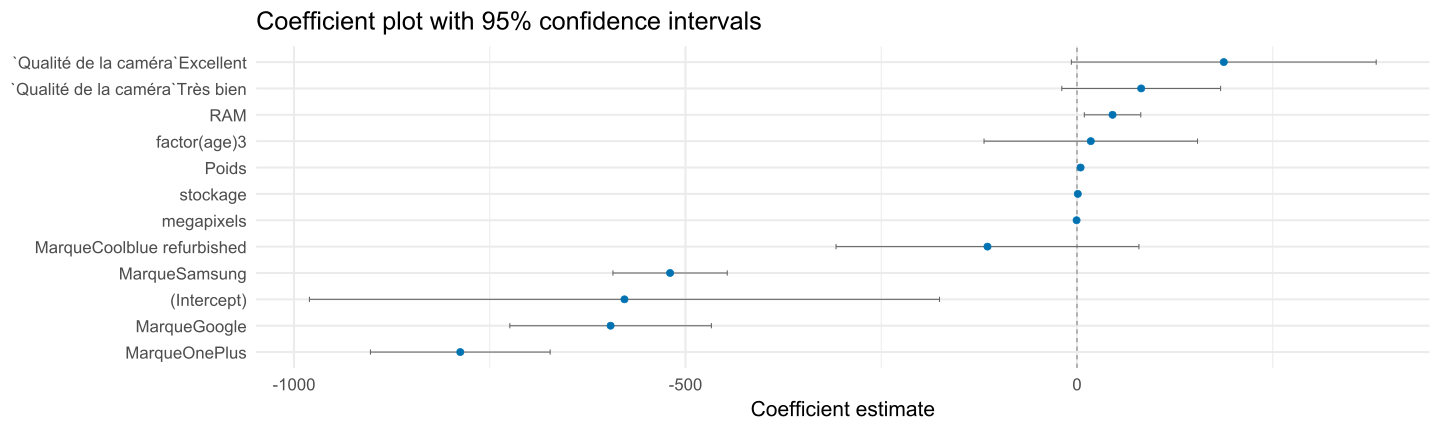
\includegraphics[keepaspectratio]{hello_files/figure-pdf/unnamed-chunk-10-1.png}}

}

\caption{Coefficients de régression hédonique}

\end{figure}%

. . .

On observe une nette différence entre les prix de Samsung / Google /
OnePlus et ceux de Apple !

\subsection{Notre régression hédonique -
IV}\label{notre-ruxe9gression-huxe9donique---iv}

Discuter ses résultats

\begin{itemize}
\tightlist
\item
  Le signe des coefficients
\item
  La forme fonctionnelle
\item
  L'expression des variables explicatives (quantitative vs qualitative)
\item
  Pourquoi observe-t-on de tels résultats ? -\textgreater{} Recherche
  contextuelle !
\item
  Comparer les marchés !

  \begin{itemize}
  \tightlist
  \item
    Une autre enseigne établit-elle des prix différents ?
  \end{itemize}
\end{itemize}

\subsection{Remarques}\label{remarques-1}

\begin{itemize}
\item
  Ceci est une méthode de récolte de données. Vous être libres de
  récolter des données autrement. Des sites recensent des jeux de
  données existantes.
\item
  Votre travail devra être rigoureusement référencé (sites, articles
  scientifiques, actualité). Tout plagiat sera sévèrement et
  indiscutablement sanctionné.
\item
  Vous êtes libres d'utiliser le logiciel statistique que vous
  préférez\ldots{} mais choisissez-le bien !
\item
  Une séance pourra être organisée pour introduire l'utilisation de
  \texttt{R} ainsi que les bonnes pratiques d'usage ainsi qu'une
  guidance pour d'éventuelles questions.
\item
  Mobilisez vos connaissances d'autres cours ! \textbf{cf.}
  \emph{Méthode et modélisation économique} \& \emph{Introduction à
  l'économétrie}
\end{itemize}

\subsection{Prochaines échéances}\label{prochaines-uxe9chuxe9ances}

\begin{itemize}
\item
  \textbf{1er mars - 23h59} : Remettre une note (1 page max) dans
  laquelle vous expliquez quel bien vous souhaitez analyser et expliquez
  comment vous construirez un jeu de données.

  \emph{{[}GRP\_{]} - Note 1 (Prix)\_NOM\_1-NOM\_2-NOM\_3.pdf}
\item
  \textbf{15 mars - 23h59} : Remettre une note dans laquelle vous
  expliquez votre avancée de récolte de données - Méthode employée,
  source, quantité de données, objectifs (2 pages max)

  \emph{{[}GRP\_{]} - Note 2 (Prix)\_NOM\_1-NOM\_2-NOM\_3.pdf}
\end{itemize}

. . .

\textbf{Bon travail !}

\subsection{Liens utiles}\label{liens-utiles}

Certains sites recensent des bases de données, notamment:

\begin{itemize}
\tightlist
\item
  \href{https://www.kaggle.com/}{Kaggle}:https://www.kaggle.com
\item
  \href{https://datasetsearch.research.google.com/}{Google Dataset
  Search}:https://datasetsearch.research.google.com
\item
  \href{https://archive.ics.uci.edu/}{UC Irvine Machine learning
  repository}:https://archive.ics.uci.edu/
\end{itemize}

/!\textbackslash{} Si vous exploitez une base de données que vous n'avez
pas constitué vous-mêmes, il est exigé de référencer dûment les auteurs
et autrices du jeu de données.

\begin{itemize}
\tightlist
\item
  \href{https://www.youtube.com/watch?v=hhqhyexDrsg}{Tutoriel vidéo
  d'installation R \& Rstudio}:
  https://www.youtube.com/watch?v=hhqhyexDrsg
\item
  \href{https://www.jetbrains.com/help/pycharm/installation-guide.html\#toolbox}{Tutoriel
  d'installation
  Pycharm}:https://www.jetbrains.com/help/pycharm/installation-guide.html\#toolbox
\item
  \href{https://www.youtube.com/watch?v=NB8OceGZGjA}{Tutoriel vidéo
  d'utilisation Selenium
  (Webscraping)}:https://www.youtube.com/watch?v=NB8OceGZGjA
\end{itemize}

\subsection{Bibliographie}\label{bibliographie}

\phantomsection\label{refs}
\begin{CSLReferences}{1}{0}
\bibitem[\citeproctext]{ref-woolridge}
Wooldridge, Jeffrey M. 2015. \emph{Introduction {à} l'{é}conom{é}trie:
Une Approche Moderne}. Louvain-La-Neuve, Belgium: De Boeck superieur.

\end{CSLReferences}




\end{document}
